% Updated in May 2014 by Hideo Saito
% Updated in March 2012 by Yasuyuki Matsushita
% Updated in April 2002 by Antje Endemann, ...., and in March 2010 by Reinhard Klette
% Based on CVPR 07 and LNCS style, with modifications by DAF, AZ and elle 2008, AA 2010, ACCV 2010

\documentclass[runningheads]{llncs}
\usepackage{graphicx}
\usepackage{amsmath,amssymb} % define this before the line numbering.
%\usepackage{ruler}
\usepackage{color}

\usepackage{epstopdf}
\usepackage{times}
\usepackage{epsfig}
\usepackage{graphicx}
\usepackage{url}
\usepackage{bm}

%===========================================================
\begin{document}
\pagestyle{headings}
\mainmatter

%===========================================================
\title{Clouds in The Cloud:\\
Supplementary Material}

\titlerunning{Clouds in The Cloud - Supplementary Material}
\authorrunning{Dmitry Veikherman, Amit Aides, Yoav Y. Schechner and Aviad Levis}

\author{Dmitry Veikherman, Amit Aides, Yoav Y. Schechner and Aviad Levis}
\institute{Dept. of Electrical Engineering, Technion - Israel Inst. of Technology, Haifa, Israel}

\maketitle
\begin{abstract}
In~\cite{danny2014} we describe simulations and an appearance consistency measure that we used. The essence is in the paper, while in this supplemental document we give more details and results.

\end{abstract}

%===========================================================
\section{Simulations}

In Sec. 8 of~\cite{danny2014} we describe simulations, which enabled us to quantitatively assess performance of 3D cloud recovery. Here we give more details.

An atmosphere over $8{\rm km}\times 8{\rm km}$  was produced using off-the-shelf UCLA large eddy simulation (LES)~\cite{stevens_evaluation_2005}. It created a field of liquid water content (LWC) per voxel, which represented clouds between heights of $500{\rm m}$ to $1500{\rm m}$. Fig.~\ref{fig:simulation_imgs2}(a) shows a $2.5\times 2.5\times 1.5{\rm km}^3$ subset of this atmosphere.
\begin{figure}
  \begin{center}
    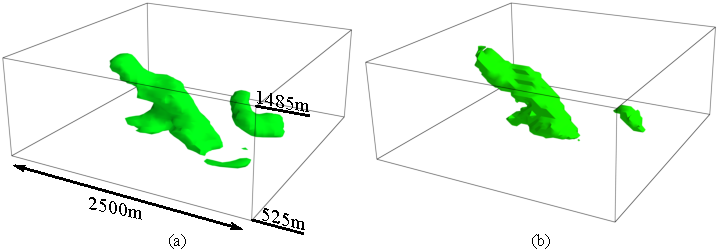
\includegraphics{clouds3d_SHDOM}
    \caption{(a) The water liquid content distribution, showing clouds in the atmosphere.
     This is a major input to SHDOM calculations. (b)
      Reconstructed clouds.}
    \label{fig:simulation_imgs2}
  \end{center}
\end{figure}
The LWC field then affected radiative transfer, calculated using the discrete ordinate spherical-harmonic method (SHDOM)~\cite{Evans1998}. The solar zenith angle was set to $\frac{\pi}{4}$.

Figs.~\ref{fig:simulation_imgs1}(a,b) show images from two out of 100
synthesized cameras. The atmosphere above the cameras is marked by red rectangles in Figs.~\ref{fig:simulation_imgs1}(a,b). The applied static Sun-blocker is tailored to solar trajectories in the latitude of Copenhagen. Figs.~\ref{fig:simulation_imgs1}(c,d) show images using the simulated Sun-blocker.
We reconstructed the cloud distribution in the atmosphere above the cameras. Fig.~\ref{fig:simulation_imgs2}(b) shows one reconstruction result, as described in~\cite{danny2014}.
\begin{figure}
  \begin{center}
    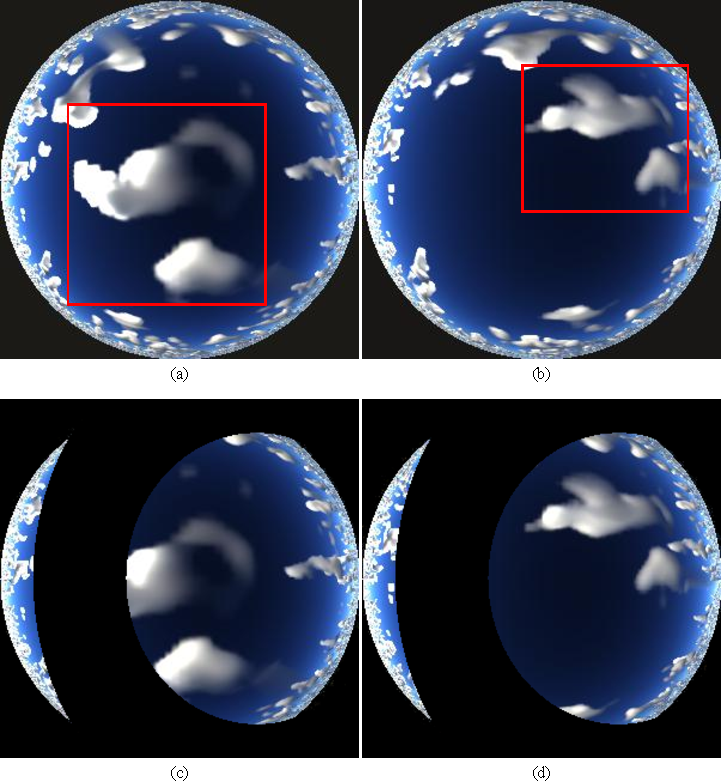
\includegraphics{simulation_imgs}
    \caption{Images synthesised using SHDOM and used in the
      reconstruction algorithm: (a,b) Two images (out of 100) of the
      same scene from different cameras. The red-marked rectangles define
      a region of interest, right above the network. (c,d) The
      same images, taken under a static sun-blocker.}
    \label{fig:simulation_imgs1}
  \end{center}
\end{figure}


\section{Appearance Consistency Score}
\label{sec:appearancecore}

In Sec.~8 of~\cite{danny2014}, we describe a matching criterion we used to demonstrate space carving of clouds. Here we give more details about it, to ease reproducibility.

Basic space carving is usually based on pointwise photo-consistency. As we explain in Sec.~8 of~\cite{danny2014}, in clouds photo-consistency is sometimes not sufficiently discriminative. Dense SIFT~\cite{liu2008sift} can be effective for non-rigid image matching. Similarly, dense SIFT can be incorporated into a space-carving scheme, to represent structural appearance of a projected voxel.
Voxel $k$ projects to a subset of the rays $\rho_k\subset{\cal R}$.
For each ray $r\in\rho_k$, we measure the radiance $\hat I_t^{\chi}(r)$ (after correcting radiometric non-uniformities), where
 $\chi\in\{{\rm R,G,B}\}$ is the color-channel index. This forms a photometric vector ${\bf v}^{\rm phot}(r,t)=[\hat I^{\rm R}_t(r),\hat I^{\rm G}_t(r),\hat I^{\rm B}_t(r)]$, which is scaled globally to a unit bound.

In addition, each ray $r$ corresponds to a pixel ${\bf x}$. From a %n $8 \times 8$
patch around ${\bf x}$, a 128-bin SIFT descriptor is extracted~\cite{lowe1999object}, yielding a vector
${\bf v}^{\rm SIFT}(r,t)$. Each such vector is normalized such that
$\|{\bf v}^{\rm SIFT}(r,t)\|_1=1$. Overall, the feature vector we use is
${\bf v}(r,t)=[{\bf v}^{\rm phot}(r,t), ~\mu{\bf v}^{\rm SIFT}(r,t)]$. Here $\mu$ determines the weight of SIFT vs. photometric descriptors. We used $\mu=1/40$ throughout the experiment. Notice that the SIFT vector contains 40 times more values, so this choise of $\mu$ gives essentially equal power to the photometric and structural properties of the patch.

Element $q$ of ${\bf v}(r,t)$ is $v_q(r,t)$. The values of this element, for all rays that intersect voxel $k$, form the set \mbox{${\cal V}_q(k,t)\equiv\{v_q(r,t)\}_{r\in\rho_k}$}.
Across viewpoints, the measured variance in this set is
${\rm VAR}[{\cal V}_q(k,t)]$.
Appearance-consistency is based on summing the variances in the different components of the feature vectors:
\begin{equation}
 P_k= \exp\left(
         -\sum_{q=1}^{131}\{{\rm VAR}[{\cal V}_q(k,t)]\}/\sigma^2
         \right)
  \;.
 \label{eq:Dist}
\end{equation}
Here $\sigma^2$ is a global scale parameter which is set to $\sigma^2=0.1$ throughout our experiments.

%\newpage
% ===========================================================
\bibliographystyle{splncs} \bibliography{cloudsbib}

% this would normally be the end of your paper, but you may also have
% an appendix within the given limit of number of pages
\end{document}
